% !TeX spellcheck = fa
\section{سوال چهارم}
در این قسمت به بررسی و مقایسه فیلتر کالمن\LTRfootnote{Kalman filter}
و فیلتر پایین گذر\LTRfootnote{Low Pass Filter}
پرداخته شده است.
در شکل
\ref{fig:real_vs_noisy}
دو سیگنال نویزی و واقعی از سیستم آورده شده است.
 \begin{figure}[H]
	\centering
	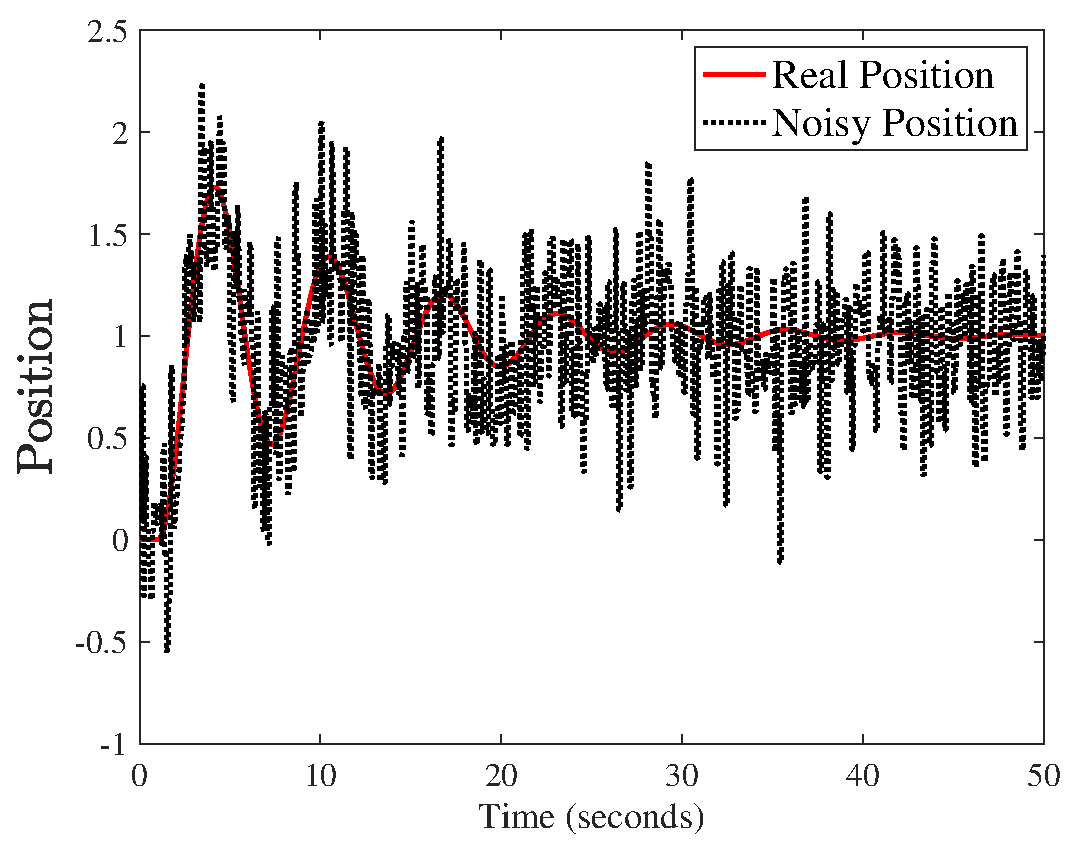
\includegraphics[width=\linewidth]{../Figure/Q4/real_vs_noisy}
	\caption{مکان واقعی و نویزی شبیه‌سازی شده}
	\label{fig:real_vs_noisy}
\end{figure}

در ادامه، برای تخمین وضعیت سیستم از بلوک آماده
\lr{Kalman Filter}
استفاده شده است. در این سیستم تنها خروجی نویزی مکان وجود دارد و هیچ داده‌ای به طور مستقیم از سرعت سیستم موجود نیست.
نتیجه پیاده‌سازی فیلتر کالمن در شکل 
\ref{fig:kalman_filter}
آمده است.

 \begin{figure}[H]
	\centering
	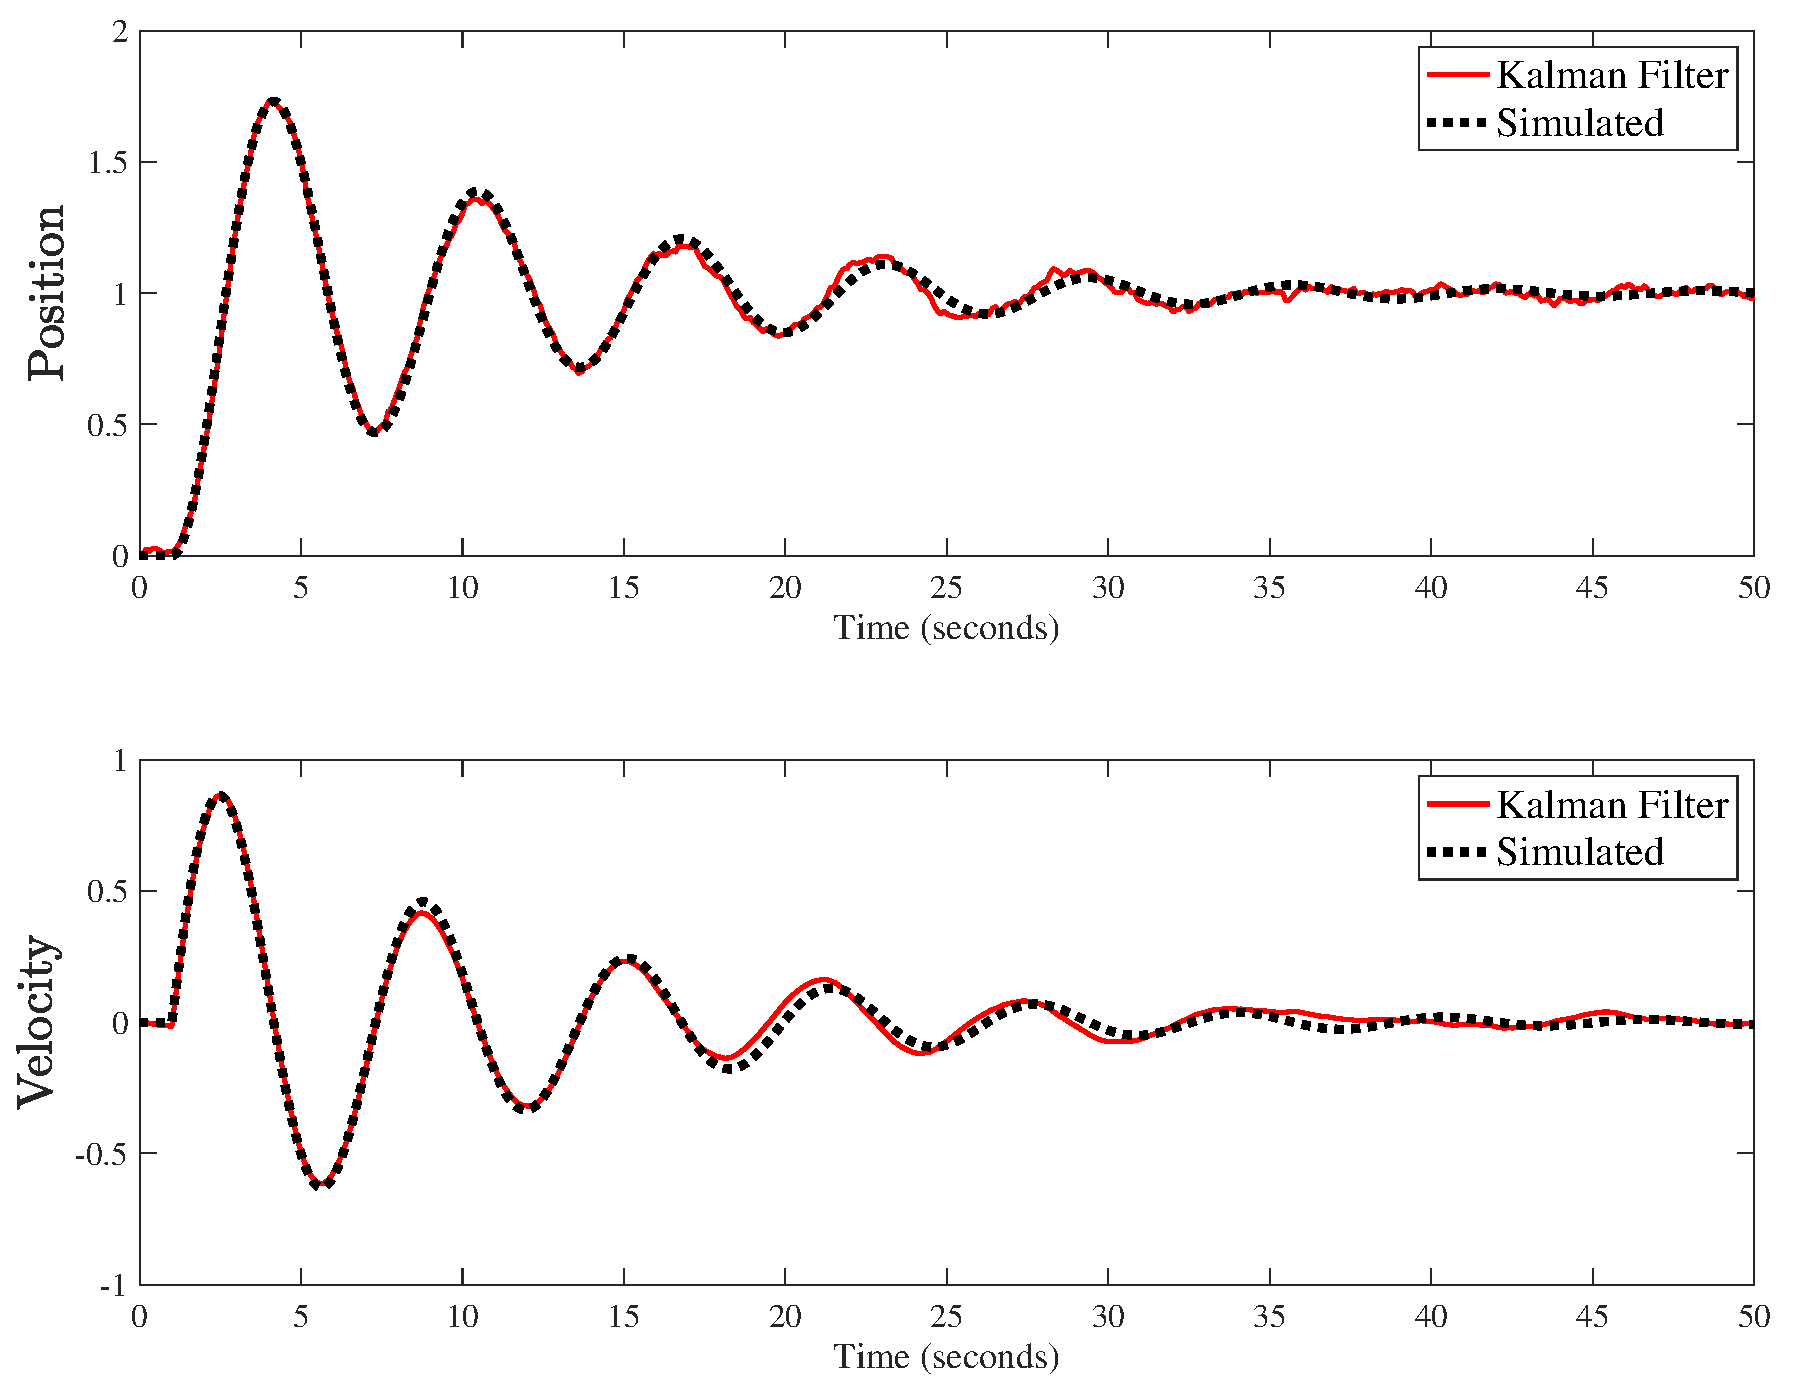
\includegraphics[width=\linewidth]{../Figure/Q4/Kalman}
	\label{fig:kalman_filter}
	\caption{مکان و سرعت تخمین زده شده با استفاده از فیلتر کالمن}
\end{figure}

در نهایت، برای تخمین وضعیت سیستم از فیلتر پایین گذر استفاده شده است.
یک تابع تبدیل برای تخمین مکان و دیگری برای تخمین سرعت با استفاده از  تابع تبدیل مشتق‌گیر به همراه فیلتر پایین گذر، استفاده است.
برای تنظیم پارامترهای فیلتر پایین گذر از روش بهینه‌سازی
\lr{Greedy}
استفاده شده است.
تابع تبدیل فیلترهای پایین گذر به صورت زیر است.
نتیجه پیاده‌سازی فیلتر پایین گذر در شکل 
\ref{fig:lpf}
آمده است.

\begin{equation}
	\text{\lr{position LPF}} = \dfrac{1}{0.5s+1}, \quad \text{\lr{velocity LPF}} = \dfrac{s}{0.5s+1}
\end{equation}
 \begin{figure}[H]
	\centering
	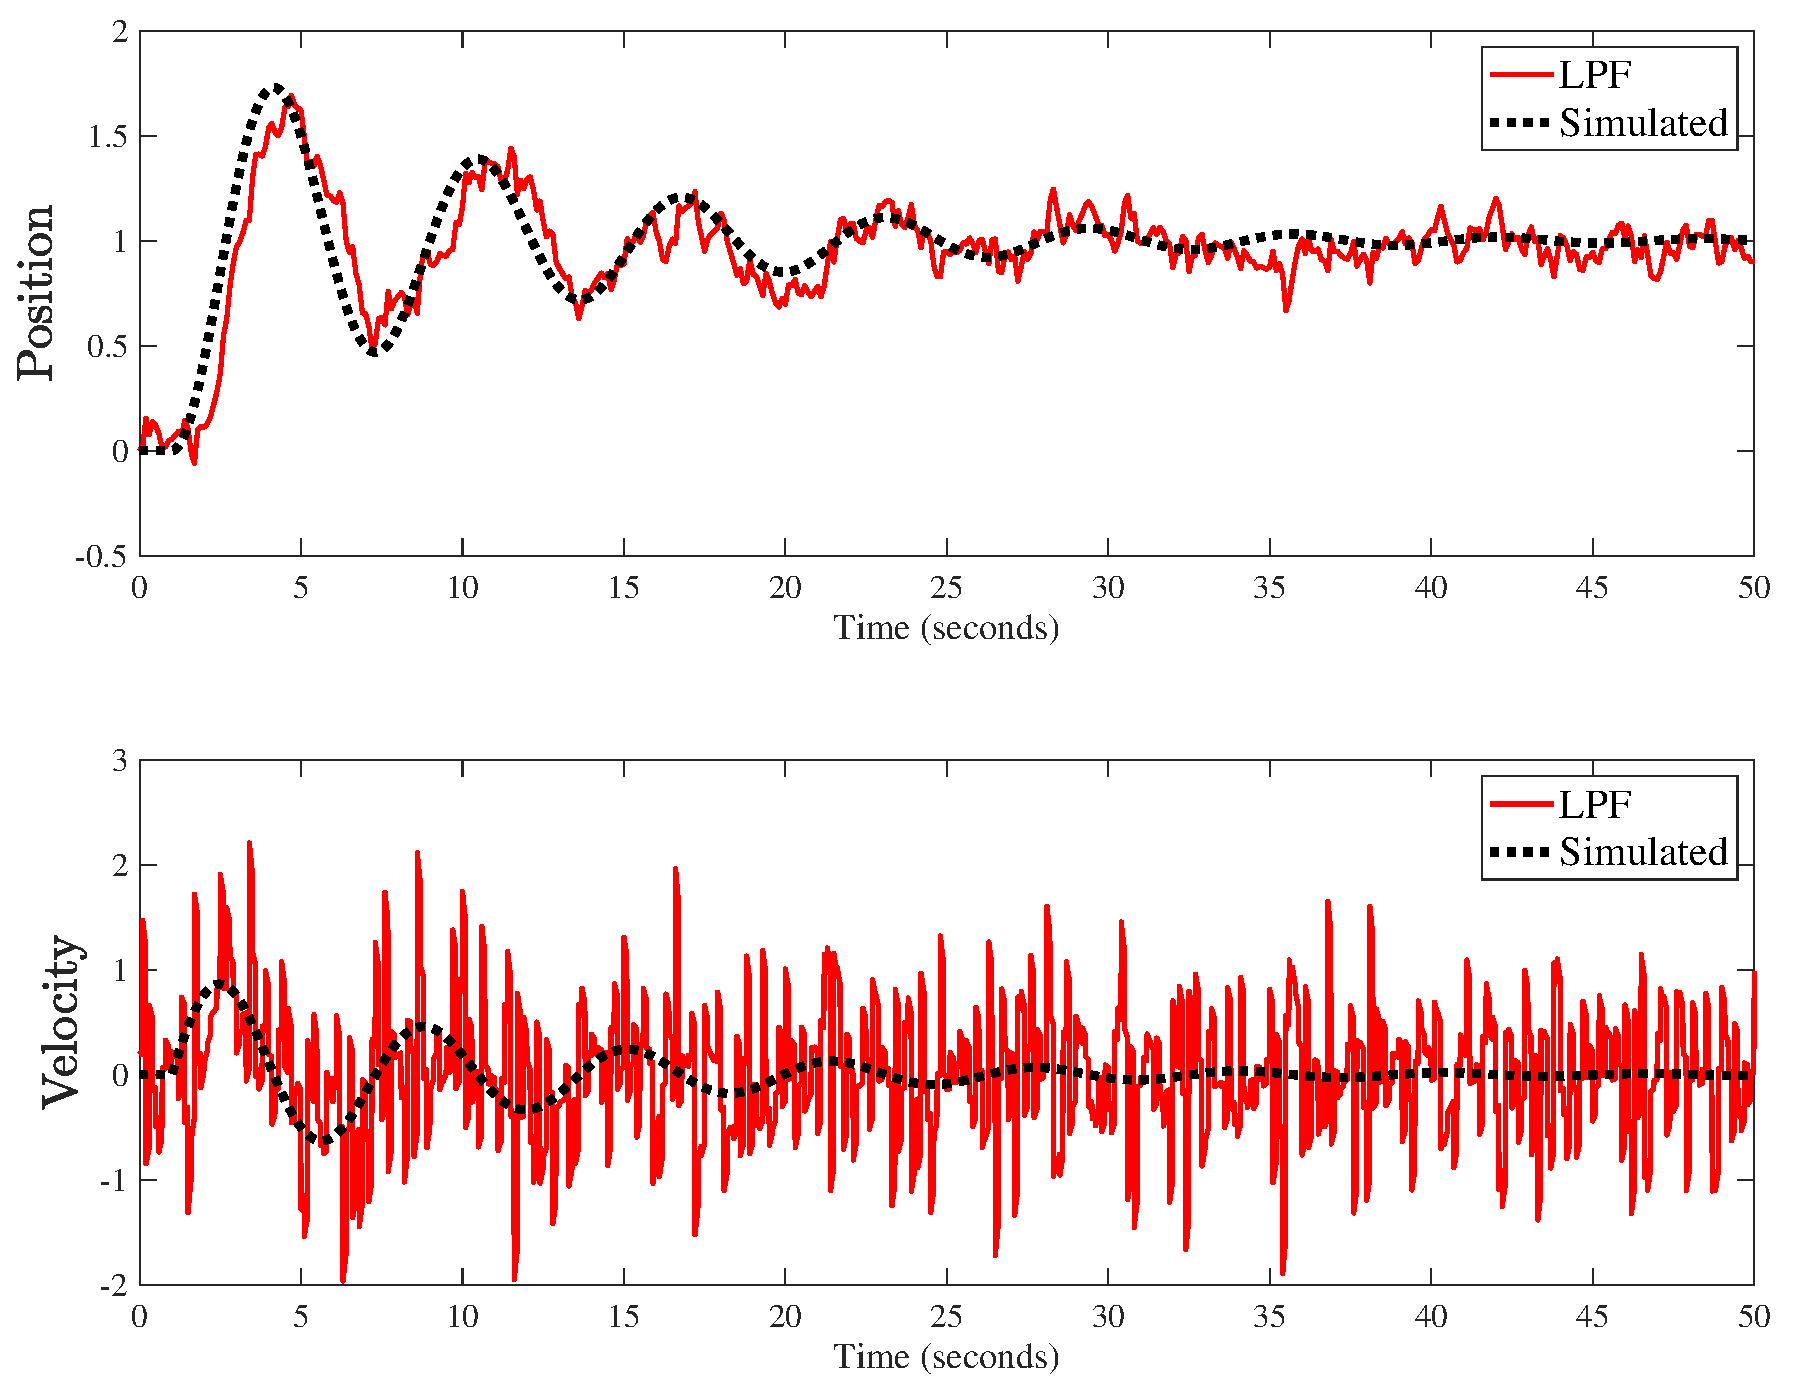
\includegraphics[width=\linewidth]{../Figure/Q4/LPF}
	\label{fig:lpf}
	\caption{مکان و سرعت تخمین زده شده با استفاده از فیلتر پایین گذر}
\end{figure}

بر اساس نتایج پیاده‌سازی، فیلتر کالمن که از مدل سیستم استفاده می‌کند، تخمین بهتر و با تاخیر کمتری می‌زند و در نهایت عملکرد بهتری نسبت به فیلتر پایین گذر دارد.

